% Research Paper for GECCO 2015
% by Nic McPhee, Kirbie Dramdahl, and David Donatucci

\documentclass{sig-alternate}

\usepackage{graphicx}
\usepackage{algorithm}
\usepackage{algpseudocode}
\usepackage{url}
\sloppy

\newcommand{\citep}[1]{\cite{#1}}

\DeclareGraphicsRule{.tif}{png}{.png}{`convert #1 `dirname #1`/`basename #1 .tif`.png}

\begin{document}

\conferenceinfo{GECCO'15,} {July 11-15, 2015, Madrid, Spain.}
\CopyrightYear{2015}
\crdata{TBA}
\clubpenalty=10000
\widowpenalty = 10000
    
\title{Impact of Crossover Bias in Genetic Programming}

\numberofauthors{1}
\author{
\alignauthor
Nicholas Freitag McPhee, M. Kirbie Dramdahl, David Donatucci\\
	\affaddr{Division of Science and Mathematics}\\
	\affaddr{University of Minnesota, Morris}\\
	\affaddr{Morris, MN USA-56267}\\
	\email{\{mcphee, dramd002, donat056\}@morris.umn.edu}
}

% This is more like how it "should" be done, but I think the previous approach might look nicer. They
% may force us to change it, though, to make it easier to scrape information.

%\numberofauthors{3}
%\author{
%\alignauthor
%Nicholas Freitag McPhee\\
%	\affaddr{Division of Science and Mathematics}\\
%	\affaddr{University of Minnesota, Morris}\\
%	\affaddr{Morris, MN USA-56267}\\
%	\email{mcphee@morris.umn.edu}
%\alignauthor
%M. Kirbie Dramdahl\\
%	\affaddr{Division of Science and Mathematics}\\
%	\affaddr{University of Minnesota, Morris}\\
%	\affaddr{Morris, MN USA-56267}\\
%	\email{dramd002@morris.umn.edu}
%\alignauthor
%David Donatucci\\
%	\affaddr{Division of Science and Mathematics}\\
%	\affaddr{University of Minnesota, Morris}\\
%	\affaddr{Morris, MN USA-56267}\\
%	\email{donat056@morris.umn.edu}
%}

\date{} 

\maketitle

\begin{abstract}

In tree-based genetic programming (GP) with sub-tree crossover, the parent contributing the root portion of the tree (the
\emph{root parent}) often contributes more to the semantics of the resulting child than the other parent (the
\emph{non-root parent}). Previous research demonstrated that when the root parent had greater fitness than the non-root
parent, the fitness of the child tended to be better than if the reverse were true. Here we explore the significance of
that asymmetry by introducing the notion of \emph{crossover bias}, which allows us to bias the system in favor of
having the more fit parent be the root parent.

Here we apply crossover bias to a variety of problems. In most cases we found that using crossover bias 
either improved performance or had no impact, although the effectiveness is somewhat dependent on the 
problem, and significantly dependent on other parameter choices, and in certainly circumstances adding
crossover bias can actually hurt performance.

While this work focuses specifically on sub-tree crossover in tree-based GP, many biological and 
artificial evolutionary systems have substantial asymmetries, many of which remain unstudied. This 
work suggests that there is probably value in exploration of the impacts of those asymmetries.

\end{abstract}

\category{}{}{}
\terms{}
\keywords{genetic programming, crossover bias, root parent}

\section{Introduction} \label{sec:Introduction}

\textbf{Comment out the authors before submission}
\textbf{Enter categories, general terms, and keywords}

As Figure~\ref{fig:root_parent_illustration} illustrates, the widely used sub-tree crossover operator in tree-based 
genetic programming (GP)~\cite{poli08:fieldguide} is an inherently
asymmetric operation, with one parent contributing the root node and, in most cases, a substantially larger
number of nodes than the other parent. This asymmetry has been noted before, e.g.,~\cite{mcphee1999analysis}
where they refer to the parent that contributes the root node as the \emph{root parent} and the other parent as
the \emph{non-root parent}.
It has also been previously observed 
\cite{burlacu2013visualization, McPheeDonatucciDramdahl:2014,  McPhee:2008:SBB:1792694.1792707} 
that the root parent often contributes more to the semantics of the resulting 
individual. This is in part because the root parent typically contributes more 
overall nodes, and because the nodes closest to the root of the tree frequently have a stronger
impact on the result of evaluating the tree in question. While the specific impact of this asymmetry depends on the details of the function set and the particular trees chosen as parents,  asymmetry has a substantial effect on the semantics of the offspring in many common 
tree-based GP settings. 

\begin{figure}
\centering
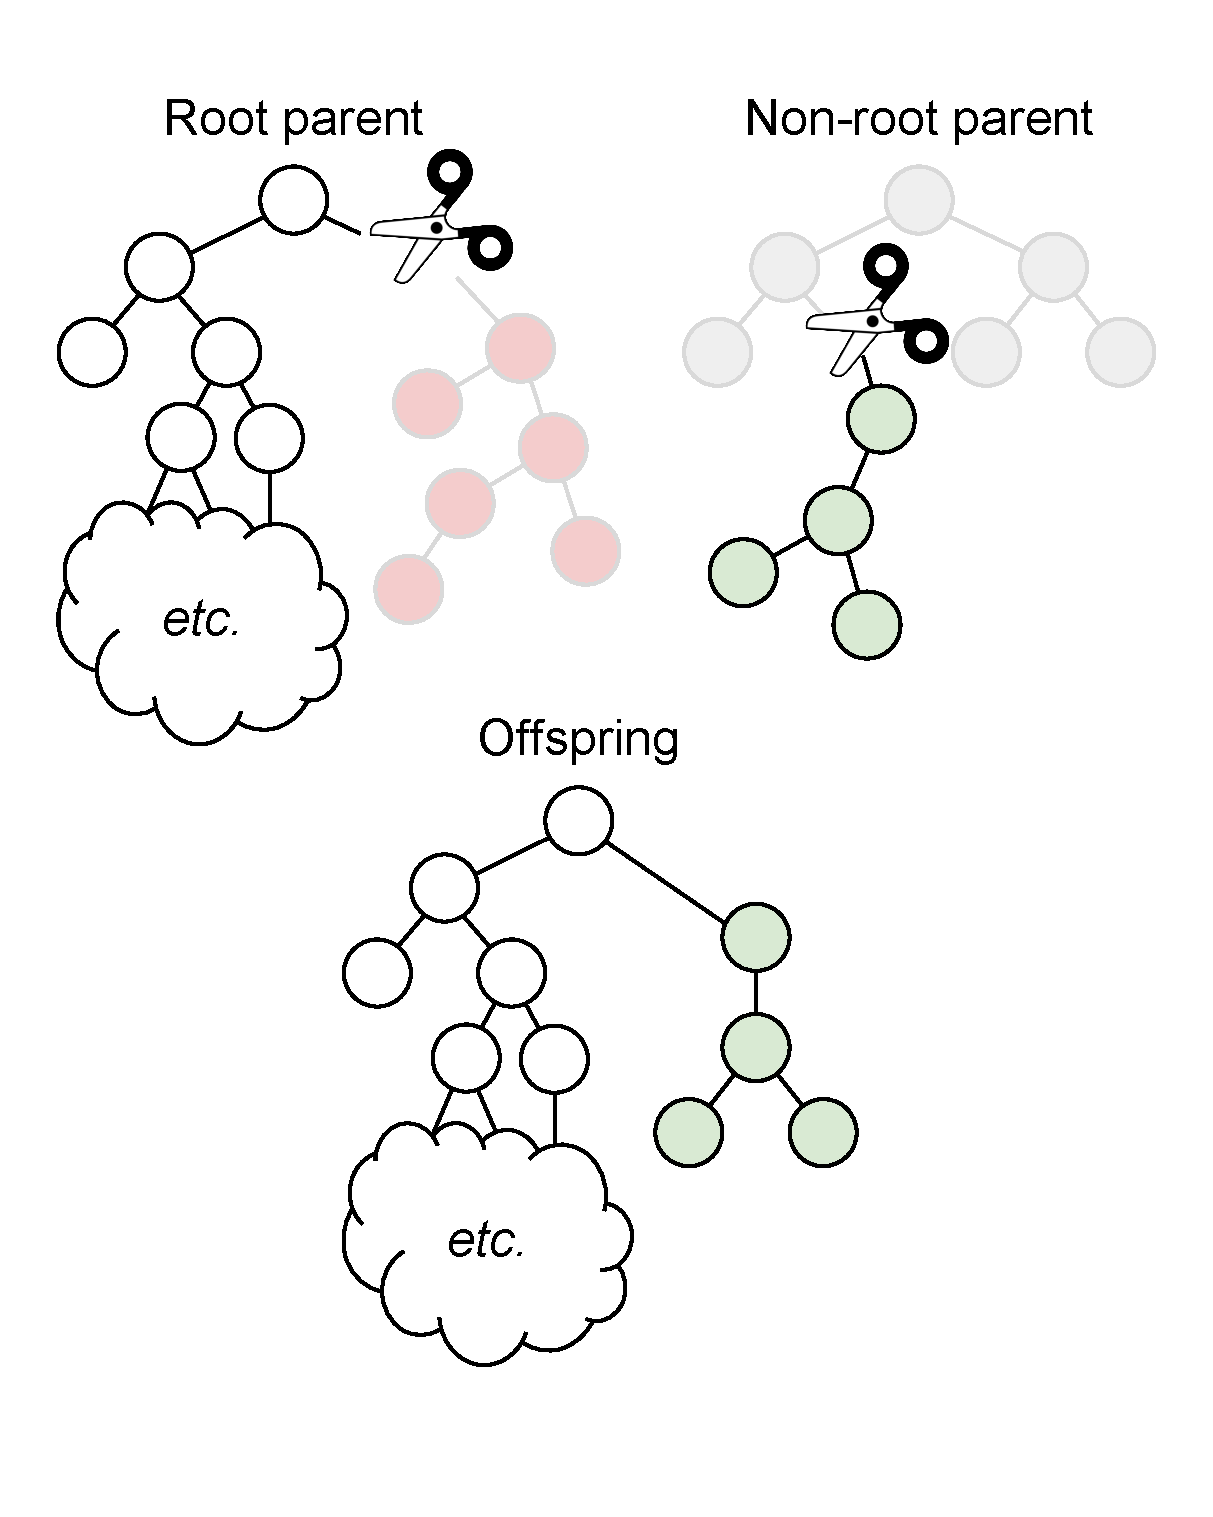
\includegraphics[width=0.45 \textwidth]{Plots/Root_parent_illustration_no_triangle.pdf}
\caption{Sub-tree crossover, illustrating the asymmetric role of the \emph{root} and \emph{non-root} parents.}
\label{fig:root_parent_illustration}
\end{figure}

An important impact of this asymmetry was recently noted in~\cite{McPheeDonatucciDramdahl:2014},
where they observed that the fitness of the offspring tended to improve when the root parent had better 
fitness than
the non-root parent.
To explore this further, we implemented what we refer to as \emph{crossover bias}, which allowed us to
probabilistically force the GP system to assign the individual with the greater 
fitness to be the root parent. In this paper, we apply crossover bias (Section~\ref{sec:XObias}) 
to a variety of test problems (Section~\ref{sec:Experiments}). The results 
(Section~\ref{sec:Results}) make it clear that crossover bias can have a substantial impact on the 
performance of GP runs, but that the results are heavily parameter dependent and, to a lesser degree 
problem dependent. In general, however, we find (Section~\ref{sec:Discussion}) that incorporating 
some crossover bias is, at least in these problems, usually either advantageous or neutral. 

\textbf{Should this next paragraph be moved the Conclusions section instead of having it here?}

While this paper focuses on asymmetry in the context of tree-based GP and sub-tree crossover, it's important to 
note that asymmetries like this are common in many evolutionary systems, both biological and artificial. Much 
eukaryote reproduction is sexual, and brings with it numerous sex-linked traits and related asymmetries; this may
play an important role in speciation~\cite{qvarnstrom2009speciation}, arguably one of the most crucial of 
biological asymmetries.
Many evolutionary computation systems other than tree-based GP also have 
significant asymmetries. Linear GP systems~\cite{brameier2007linear} and stack-based GP 
systems~\cite{spector:2002:GPEM}, for example, have asymmetries where the last instructions executed can have a 
disproportionate impact on the results. Similarly, changes near the front of grammatical evolution 
\cite{o2003grammatical} strings will have a 
disproportionate impact by determining the important early choices in the grammar productions. 
The results presented here suggest that it may be important to more thoroughly explore the impact of these asymmetries, both to better understand the performance and behavior of existing systems, but also as an aid to the design and discovery of new tools like recombination operators that leverage these asymmetries.

\section{Crossover Bias} \label{sec:XObias}

For this work, we implemented crossover bias with a parameter specifying the probability of forcing 
the more fit parent to be the root parent when performing crossover, as detailed in 
Algorithm~\ref{alg:biasAlgorithm}. Every time a 
crossover event was to be performed, we would use this probability to decide whether to force the 
more fit parent to be the root parent. Note that if the random value in Algorithm~\ref{alg:biasAlgorithm} 
didn't cause crossover bias to be applied, then the parents were left in their original random order, 
meaning that there is a 50\% chance that the root 
parent is the more fit parent even without any crossover bias.

\begin{algorithm}[tb]
\begin{algorithmic}
\Require Two individuals, RP (root parent) and NRP (non-root parent), are chosen as parents.
\If {\Call{random}{0, 1} $\leq \textrm{XO\_bias}$} \Comment{Do we force bias?}
    \If {\Call{fitness}{RP} \textrm{worse than} \Call{fitness}{NRP}}
        \State RP, NRP := NRP, RP \Comment{Swap so RP is more fit} 
    \EndIf
\EndIf
\end{algorithmic}
\caption{Crossover bias}
\label{alg:biasAlgorithm}
\end{algorithm}

In this paper we focus on five levels of crossover bias:
\begin{itemize}
\item 0.00 bias - no crossover bias is applied;
\item 0.25 bias - system forced to use the more fit parent as the root parent in 25\% of cases;
\item 0.50 bias - system forced to use the more fit parent as the root parent in 50\% of cases;
\item 0.75 bias - system forced to use the more fit parent as the root parent in 75\% of cases; and
\item 1.00 bias - system forced to always use the more fit parent as the root parent, sometimes referred to as ``with crossover bias''.
\end{itemize}
The 0.00 case, where no crossover bias is applied, is just standard sub-tree crossover, where there will be a 50\% chance of the root parent being the more fit parent.

We also experimented with \emph{reverse bias}, where the weaker parent was always forced to be 
the root parent. In general, the results for reverse bias revealed that there wasn't any statistically significant difference from 
no bias, so in the 
interest of simplification we've omitted reverse bias from the remainder of the paper.

\section{Experimental Setup} \label{sec:Experiments}

To better understand the impact of crossover bias on GP performance, we 
experimented with five problems: K Landscapes with $K=6$~\cite{vanneschi2011k}, 
ORDER\-TREE~\cite{hoang2006ordertree}, U.S. Change, Sine regression~\cite{poli08:fieldguide}, 
and Pagie-1 regression~\cite{pagie1997evolutionary}.
Three of these (K Landscapes, ORDERTREE, and Pagie-1 regression) are taken from recent benchmark 
suggestions~\cite{gp-benchmarks-2013}. U.S. Change is a program synthesis problem  that has proven 
interesting for evolutionary program synthesis~\cite{zhan2014quantitative}, and sine regression 
is the example problem used in earlier work on the impact of root and non-root 
parents~\cite{McPheeDonatucciDramdahl:2014}.

The one problem not precisely described elsewhere in the literature is the U.S. Change problem, 
where the task is to take as input an amount, and to return as output the minimum 
number of coins required to make that amount using (a subset of) standard U.S. coins with amounts 
25, 10, 5, and 1. So, for example, given 118 as input, the result should be 9 since 
\[
	\underline{4} \times 25 + \underline{1} \times 10 + \underline{1} \times 5 + \underline{3} \times 1 = 118,
\]
and this set of $4+1+1+3 = 9$ coins is the minimal set 
making a total of 118. Our function set for this problem was +, -, $\times$, \%,\footnote{Protected integer 
division (quotient), returning 1 if the denominator is 0.} \emph{mod}, \emph{min}, and \emph{max}. 
The terminal set consisted of the input $x$, integer ephemeral random constants taken uniformly 
from the range $[-50, 50]$, and the set of constants $\{ 0, 1, 4, 5, 9, 10, 24, 25 \}$. The test cases 
were all inputs in the range $[0, 150)$.

% This is all taken from Tom Helmuth's version of the problem, and if the paper is accepted we should credit him in the camera ready copy.

All our experiments used the previously published
settings, function sets, etc., with the exception of the parameters listed in 
Table~\ref{tab:sharedParameters},\footnote{The function 
set for Pagie-1 specified in~\cite{pagie1997evolutionary} is simply +, -, $\times$, and \% (protected division). 
The function set given in~\cite{mcdermott2012genetic} and implemented in ECJ is ``koza2'', which 
also includes various trigonometric and logarithmic functions. The performance of GP varies 
substantially between the two function sets; here we follow the original Pagie-1 paper and use the 
simpler function set.}
which are shared throughout these experiments. Our evolutionary system is 
generational, with all new individuals being generated via subtree crossover (i.e., no mutation or reproduction) 
unless there is a non-zero elitism percentage. Our primary goal was to better understand the 
impact of crossover bias, so we performed runs with a variety of crossover bias probabilities. In addition,  we
wanted to see how crossover bias might interact with some other commonly manipulated parameters 
as listed in Table~\ref{tab:sharedParameters}. Unless otherwise noted, all plots, etc., in what follows will include results from 
all possible combinations of values in Table~\ref{tab:sharedParameters}. Each box plot in 
Figure~\ref{fig:KLandscapes6_results}, for example, includes the results of 100 runs for each of the 
combinations of all four 
tournament sizes, both elitism proportions, and both population sizes.

\begin{table}[tb]
\begin{center}
\begin{tabular}{ll}
\textbf{Parameter} & \textbf{Values} \\
% \hline
Crossover bias & 0, 0.25, 0.5, 0.75, and 1 \\
Tournament size & 2, 3, 5, and 7 \\
Elitism \% & 0 and 1\% (\& sometimes 0.1\%) \\
Population size & 1,024 and 10,240 \\
\# of generations & 100 \\
\# of runs per treatment & 100
\end{tabular}
\end{center}
\vspace{-0.5cm}
\caption{Shared parameters}
\label{tab:sharedParameters}
\end{table}

\textbf{Can we drop 0.1\% from the table and just handle it as an exception like Tarpeian?}

As Section~\ref{sec:Results} shows, there were some quite substantial interactions between 
crossover bias and some of the other parameter settings. In particular, we found that there are 
parameter values where crossover bias appears to have a substantial and significant impact, 
and other parameter settings
where crossover bias has almost no effect on the results. 
Based on these observed patterns, 
we found it useful to identify two specific subsets of the parameter settings listed in 
Table~\ref{tab:sharedParameters}: ``\emph{bias-effective settings}'' and 
``\emph{non-bias-effective settings}''.
The bias-effective settings are binary tournaments, no elitism, and population size of 10,240; 
the non-bias-effective settings, conversely, are tournament size 7, non-zero elitism percentage, 
and population size 1,024. These terms will be used in the remainder of the paper, which will 
also include some discussion of why crossover bias might interact with these parameters in this way.

All experiments were run using a copy of ECJ 21\footnote{\url{http://cs.gmu.edu/~eclab/projects/ecj/}} 
that we modified to support crossover bias.

\section{Results} \label{sec:Results}

All tests of differences in fitness or hits in this section are performed using 
pairwise Wilcoxon tests with Holm corrections. Tests of differences in the number of successes are
performed using pairwise tests of proportions (chi-squared) with Holm corrections.
All statistics calculations were performed with R~\cite{R} 
and plots were generated using the\linebreak ggplot2 package~\cite{ggplot2Book}.

\subsection{Structural Problems}

\textbf{Someone should invent a sentence to put here.}

\subsubsection{K Landscapes}

Figure~\ref{fig:KLandscapes6_results} shows the impact of crossover bias on this problem across all the combinations of
parameter values in Table~\ref{tab:sharedParameters}. Increasing the amount of crossover bias consistently improves the fitness of the results. All the
differences are statistically significant ($p < 0.012$) except for the difference between bias probability 0.75 and
1.00.

%> pairwise.wilcox.test(klandscapes6$Fitness, klandscapes6$Bias.probability)
%
%	Pairwise comparisons using Wilcoxon rank sum test 
%
%data:  klandscapes6$Fitness and klandscapes6$Bias.probability 
%
%     -1      0       0.25    0.5     0.75   
%0    0.99997 -       -       -       -      
%0.25 1.8e-06 1.8e-06 -       -       -      
%0.5  1.7e-12 2.3e-12 0.01136 -       -      
%0.75 < 2e-16 < 2e-16 6.0e-10 0.00032 -      
%1    < 2e-16 < 2e-16 3.7e-15 2.2e-07 0.15773
%
%P value adjustment method: holm 

\begin{figure}
\centering
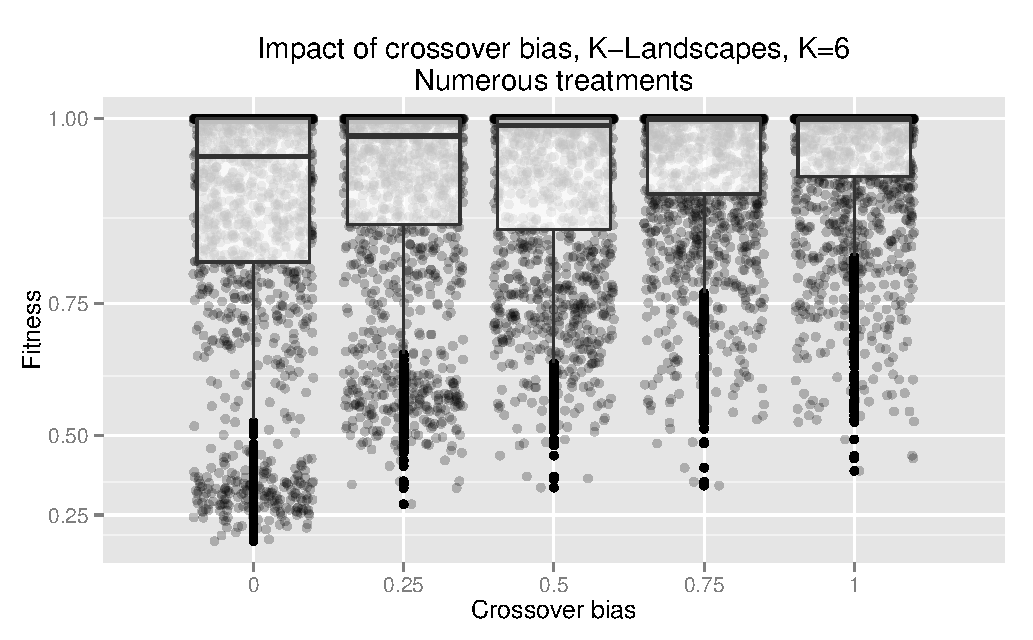
\includegraphics[width=0.45 \textwidth]{Plots/KLandscapes6_XO_bias_impact_transformed_boxplot_alpha075.pdf}
\caption{Impact of crossover bias on fitness for K Landscapes problem, for a variety of treatments.}
\label{fig:KLandscapes6_results}
\end{figure}

Compare this to the results shown in Figure~\ref{fig:KLandscapes6_XO_bias_impact_facets}, which plots the same data
separated out by tournament size. It is clear that for binary tournaments, increasing the crossover bias probability
continues to improve the fitness -- all the differences are strongly statistically significant ($p<6\times 10^{-08}$). This
continues to be true for tournament size 3; all the differences are statistically significant except for those between
bias 0.50 and 0.75, which was very close ($p=0.05620$). None of the differences for tournament size 5 are
significant. For tournament size 7, however, it does look like the reverse is true, where
increasing crossover actually hurts fitness. Almost none of the differences for tournament size 7 are statistically
significant, however, with the only exception being the difference between 0.25 and 1.00 ($p=0.21$).

\textbf{Nic needs to check the p=0.21 above since that clearly isn't signifiant. Either Nic was confused, or the number should be 0.021.}

\begin{figure}
\centering
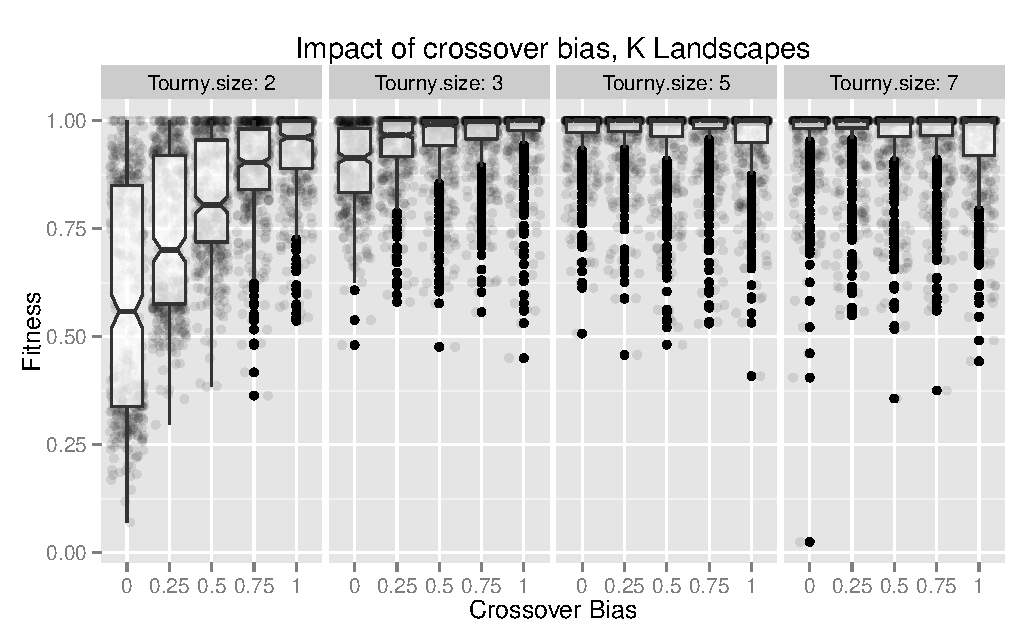
\includegraphics[width=0.45 \textwidth]{Plots/KLandscapes6_XO_bias_impact_facets.pdf}
\caption{Impact of crossover bias on fitness for K Landscapes problem, for various tournament sizes.}
\label{fig:KLandscapes6_XO_bias_impact_facets}
\end{figure}

\textbf{Take hyphen out of K Landscapes graph titles, and remove K=6.}

Figure~\ref{fig:KLandscapes6_strong_results} filters out only the data gathered using the bias-effective treatment,
discussed in Section~\ref{sec:Experiments}. It is clear that the impact of crossover bias is much stronger in this case
than in the more general case shown in Figure~\ref{fig:KLandscapes6_results}. Here all the differences are strongly
statistically significant ($p < 10^{-11}$). In addition to improvements in fitness, increasing the crossover bias also
increases the number of ``perfect'' solutions discovered. Out of 100 runs with a crossover bias setting of 1.00, 15 of
these runs resulted in the discovery of a ``perfect'' solution. By comparison, only 1 or 2 runs out of 100 resulted in
``perfect'' solutions for each of the other crossover bias probabilities. This difference is statistically significant with
$p \leq 0.03$.

\begin{figure}
\centering
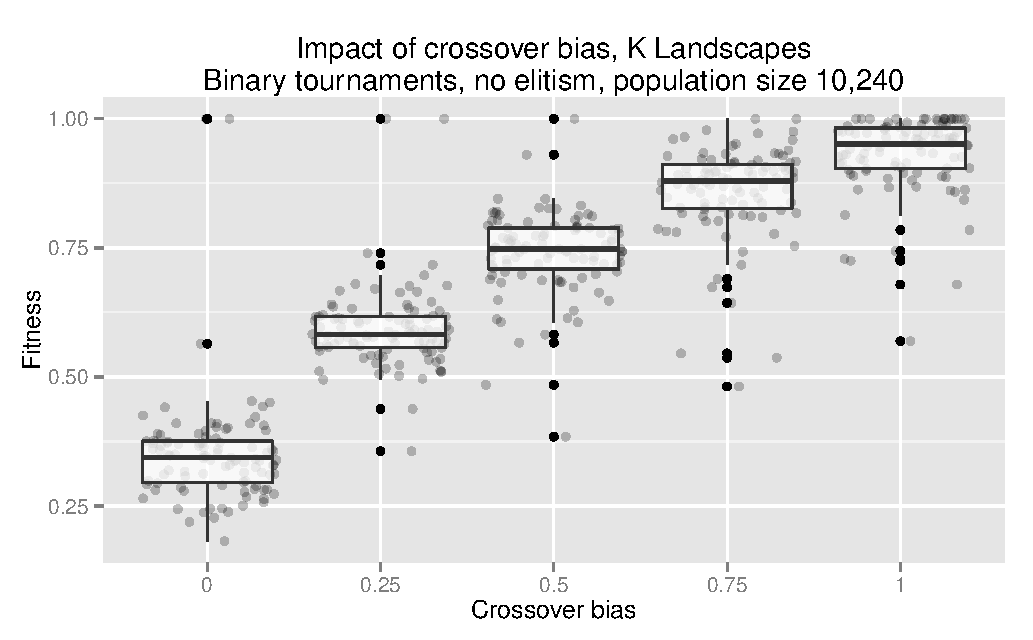
\includegraphics[width=0.45 \textwidth]{Plots/KLandscapes6_XO_bias_strong_impact_alpha_075.pdf}
\caption{Impact of crossover bias on fitness for K Landscapes problem, restricted to bias-effective parameter settings.}
\label{fig:KLandscapes6_strong_results}
\end{figure}

%> pairwise.wilcox.test(strong$Fitness, strong$Bias.probability)
%
%	Pairwise comparisons using Wilcoxon rank sum test 
%
%data:  strong$Fitness and strong$Bias.probability 
%
%     -1      0       0.25    0.5     0.75   
%0    0.18    -       -       -       -      
%0.25 < 2e-16 < 2e-16 -       -       -      
%0.5  < 2e-16 < 2e-16 < 2e-16 -       -      
%0.75 < 2e-16 < 2e-16 < 2e-16 < 2e-16 -      
%1    < 2e-16 < 2e-16 < 2e-16 < 2e-16 2.3e-12
%
%P value adjustment method: holm 

%> countSuccesses(strong)
%[1]  1  2  2  1  2 15
%> pairwise.prop.test(countSuccesses(strong), rep(100, 6))
%
%	Pairwise comparisons using Pairwise comparison of proportions 
%
%data:  countSuccesses(strong) out of rep(100, 6) 
%
%  1     2     3     4     5    
%2 1.000 -     -     -     -    
%3 1.000 1.000 -     -     -    
%4 1.000 1.000 1.000 -     -    
%5 1.000 1.000 1.000 1.000 -    
%6 0.011 0.030 0.030 0.011 0.030
%
%P value adjustment method: holm 

\subsubsection{ORDERTREE}

It should be noted that, for the ORDERTREE problem we used the full set of parameters outlined in
Section~\ref{sec:Experiments}, with one exception: the population size for the ORDERTREE 
runs was limited to 1,024.
This was a consequence of the large trees generated for this problem, resulting in out of memory errors for the larger
population size of 10,240.

Initial runs of this problem with (1.00) and without (0.00) crossover bias across all four tournament sizes
demonstrated that in each case, adding crossover bias improved fitness. Additionally, these improvements were
statistically significant ($p < 0.002$).

Figure~\ref{fig:Ordertree_results_all_tournaments_Jan15} generalizes this to cover the full range of 
crossover bias
percentages, and shows a more complex picture. 
For binary tournaments, we observed a drop in fitness from bias 0.75 to bias 1.00, where the fitness for
1.00 is actually slightly below that for 0.50 as well. All these differences are statistically significant ($p <
0.03$), with the exception of the difference between bias 0.25 and bias 1.00, so bias 0.75 is the clear winner in this
scenario. This drop in fitness for bias 1.00
is consistent across the other three tournament sizes as well. However, it is also
apparent from the figure that in general the impact of crossover bias lessens with the larger tournament sizes, both in
the increase in fitness up to bias 0.75, and the drop from there to bias 1.00.

\begin{figure}
\centering
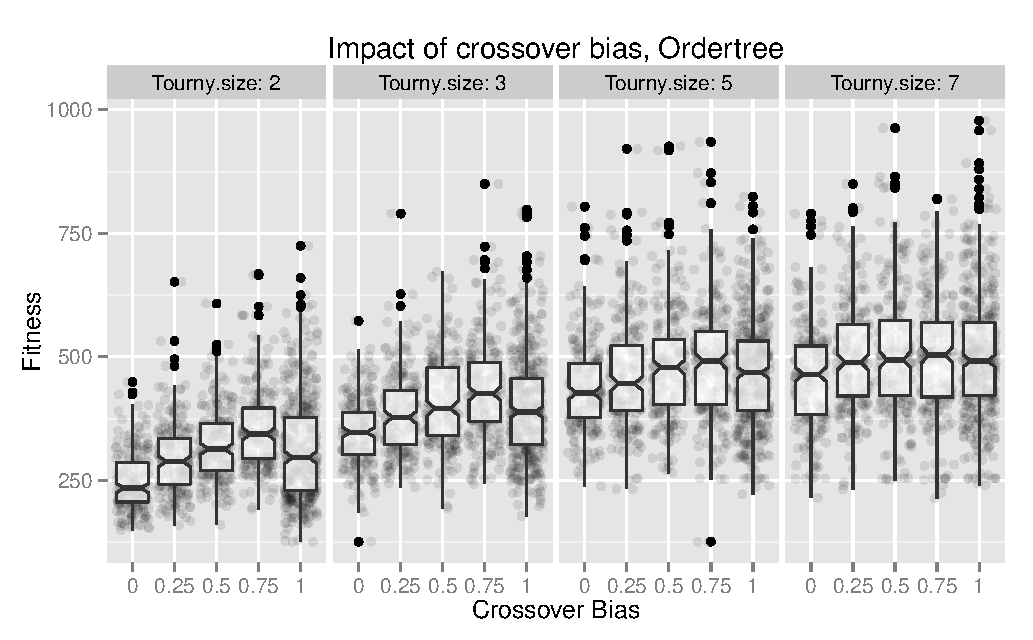
\includegraphics[width=0.45 \textwidth]{Plots/Ordertree_results_all_tournaments_Jan15.pdf}
\caption{Impact of crossover bias on fitness for ORDERTREE problem for multiple tournament sizes.}
\label{fig:Ordertree_results_all_tournaments_Jan15}
\end{figure}

\textbf{Change caps on ORDERTREE in figure titles.}

%> pairwise.wilcox.test(subset(klandscapes6, Tourny.size==7)$Fitness, subset(klandscapes6, Tourny.size==7)$Bias.probability)
%
%	Pairwise comparisons using Wilcoxon rank sum test 
%
%data:  subset(klandscapes6, Tourny.size == 7)$Fitness and subset(klandscapes6, Tourny.size == 7)$Bias.probability 
%
%     0     0.25  0.5   0.75 
%0.25 1.000 -     -     -    
%0.5  1.000 1.000 -     -    
%0.75 1.000 0.556 1.000 -    
%1    0.075 0.021 0.556 1.000
%
%P value adjustment method: holm 

\subsection{U.S. Change Problem}

In contrast to the structural problems discussed in the previous section, which used fitness as the measure of success
of a run, for the U.S. Change problem we measured success in ``hits'' (the number of test cases that are correctly
solved). There are 150 test cases in our implementation, so an optimal program will have a score of 150 hits.

Figure~\ref{fig:USChange_Hits} shows the impact of crossover bias on the number of hits for the U.S. Change problem
across the full collection of parameter settings. This suggests that in general there is little consistent impact of
crossover bias; while most of the differences in this
plot are not statistically significant, two are: the differences between crossover bias 0.00 and crossover bias 0.50 and
0.75 are both statistically significant ($p \leq 0.015$), even if numerically small.

\begin{figure}
\centering
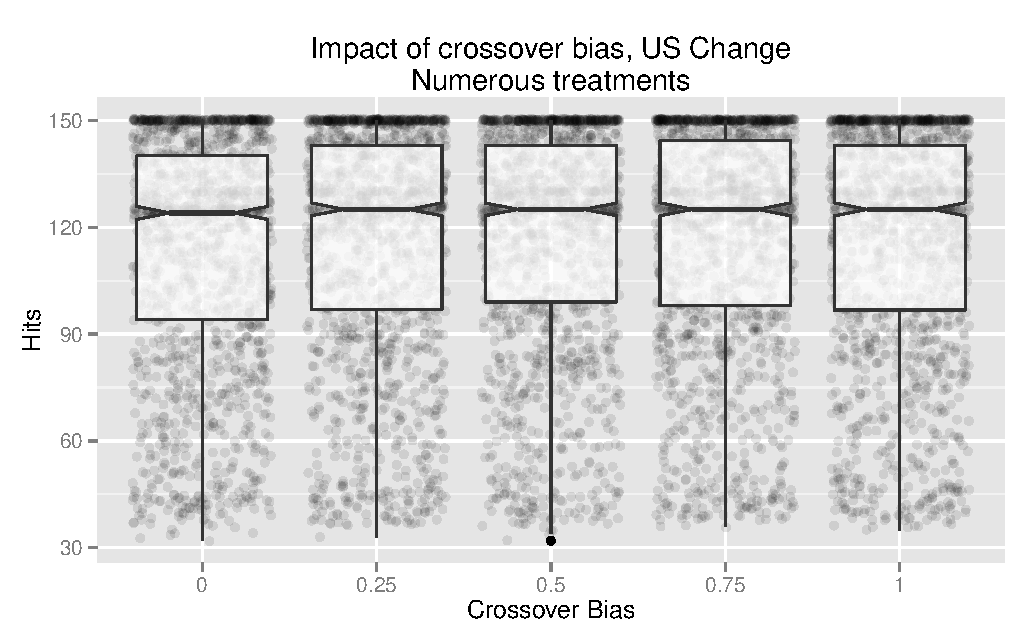
\includegraphics[width=0.45 \textwidth]{Plots/US_change_hits.pdf}
\caption{Impact of crossover bias on the number of hits for the U.S. Change problem across a variety of treatments.}
\label{fig:USChange_Hits}
\end{figure}

%> pairwise.wilcox.test(us_change$Hits, us_change$Bias, conf.int=TRUE)
%
%	Pairwise comparisons using Wilcoxon rank sum test 
%
%data:  us_change$Hits and us_change$Bias 
%
%     0     0.25  0.5   0.75 
%0.25 0.117 -     -     -    
%0.5  0.011 1.000 -     -    
%0.75 0.015 1.000 1.000 -    
%1    0.083 1.000 1.000 1.000
%
%P value adjustment method: holm 

However, if we limit our attention to the bias-effective parameter settings (Section~\ref{sec:Experiments}), then we
find that crossover bias has a substantial and statistically significant impact, as is seen in
Figure~\ref{fig:USChange_Hits_strong}. Here the bulk of these pairwise differences are statistically significant
($p<0.0002$). The major exception is the difference between
crossover bias 0.75 and 1.00 ($p=0.43078$). Two other adjacent pairs have $p$-values slightly above 0.05: crossover bias
0.25 \emph{vs} 0.50 ($p=0.05036$), and 0.50 \emph{vs} 0.75 ($p=0.08019$).

\begin{figure}
\centering
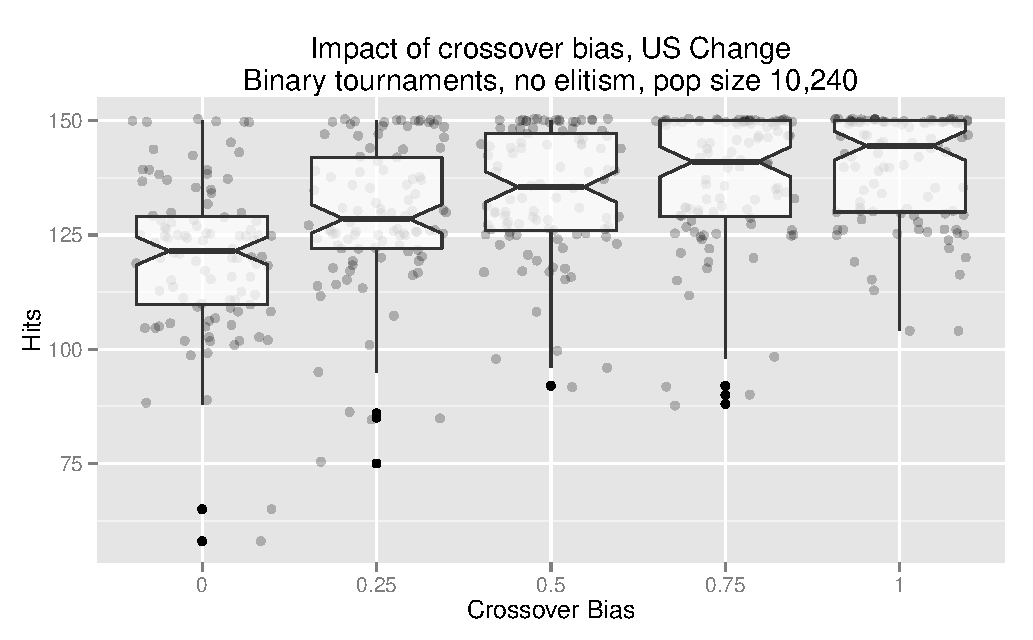
\includegraphics[width=0.45 \textwidth]{Plots/US_change_hits_strong.pdf}
\caption{Impact of crossover bias on the number of hits for the U.S. Change problem, limited to bias-effective parameters.}
\label{fig:USChange_Hits_strong}
\end{figure}

%> pairwise.wilcox.test(us_change_strong$Hits, us_change_strong$Bias)
%
%	Pairwise comparisons using Wilcoxon rank sum test 
%
%data:  us_change_strong$Hits and us_change_strong$Bias 
%
%     0       0.25    0.5     0.75   
%0.25 0.00013 -       -       -      
%0.5  3.4e-09 0.05036 -       -      
%0.75 1.1e-12 0.00016 0.08019 -      
%1    3.2e-15 5.1e-06 0.01652 0.43078
%
%P value adjustment method: holm 

If complete success was considered vital (which might be the case if we were evolving software for use in a production
system), then it would make sense to see if crossover bias has a significant impact on the success rate.
Figure~\ref{fig:USChange_Successes_strong} shows the number of successes for the various crossover bias values when
using the bias-effective parameter settings. None of the adjacent differences (for example, crossover bias 0.50 \emph{vs} 0.75)
are statistically significant, while most of the non-adjacent differences (for example, crossover bias 0.25 \emph{vs} 0.75)
are statistically significant, with the exceptions being crossover bias 0.00 \emph{vs} 0.50, and bias 0.50 \emph{vs} 1.00
($p=0.09361$ in both cases).

\begin{figure}
\centering
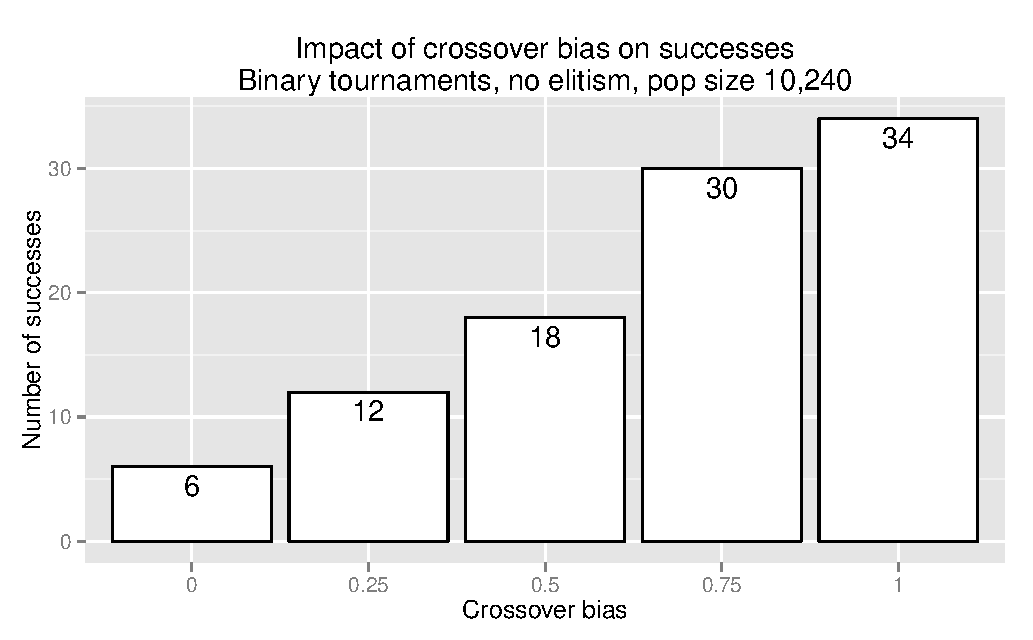
\includegraphics[width=0.45 \textwidth]{Plots/US_change_successes_strong.pdf}
\caption{Impact of crossover bias on the number of successes runs for the U.S. Change problem when using to bias-effective parameters.}
\label{fig:USChange_Successes_strong}
\end{figure}

%> pairwise.prop.test(c(6, 12, 18, 30, 34), rep(100, 5))
%
%	Pairwise comparisons using Pairwise comparison of proportions 
%
%data:  c(6, 12, 18, 30, 34) out of rep(100, 5) 
%
%  1       2       3       4      
%2 0.65003 -       -       -      
%3 0.09361 0.65003 -       -      
%4 0.00021 0.02215 0.27429 -      
%5 1.8e-05 0.00334 0.09361 0.65003
%
%P value adjustment method: holm 

%\begin{figure}
%\centering
%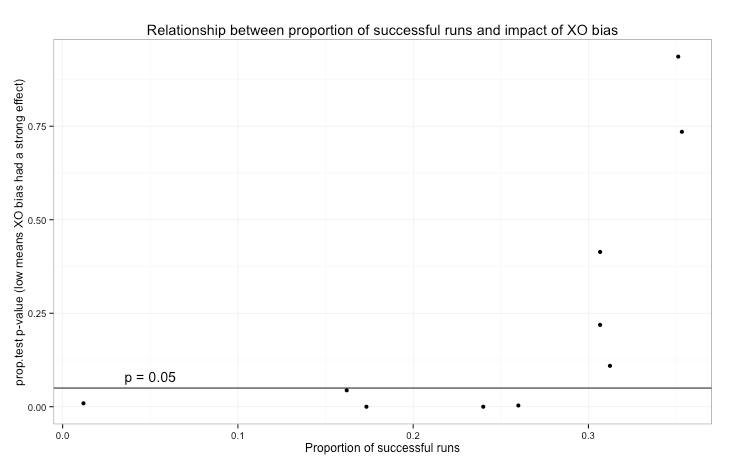
\includegraphics[width=0.45 \textwidth]{Plots/US_change_Bias_impact_vs_success.png}
%\caption{Relationship between proportion of successful runs and the impact of crossover bias.}
%\label{fig:USChangeBiasImpactVsSuccess}
%\end{figure}

\subsection{Symbolic Regression Problems}

\subsubsection{Pagie-1 Problem}

In addition to the parameters outlined in Section~\ref{sec:Experiments}, the Pagie-1 problem was also run with the ``basic4'' ($+, -, \times, \div$) function set, and with and without Tarpeian bloat control.

Figure~\ref{fig:Pagie1Hits_Bias_Tournys_FunctionSet} shows the impact of crossover bias on the number of hits for the
Pagie-1 regression problem, separated out by both tournament size and function set used. The results, as 
can be seen in Figure~\ref{fig:Pagie1Hits_Bias_Tournys_FunctionSet}, vary significantly. However, if limited 
to population size 10,240 and no elitism then the complexities of 
Figure~\ref{fig:Pagie1Hits_Bias_Tournys_FunctionSet} simplify to
Figure~\ref{fig:Pagie1StrongHits_Bias_Tournys_FunctionSet}.

\begin{figure}
\centering
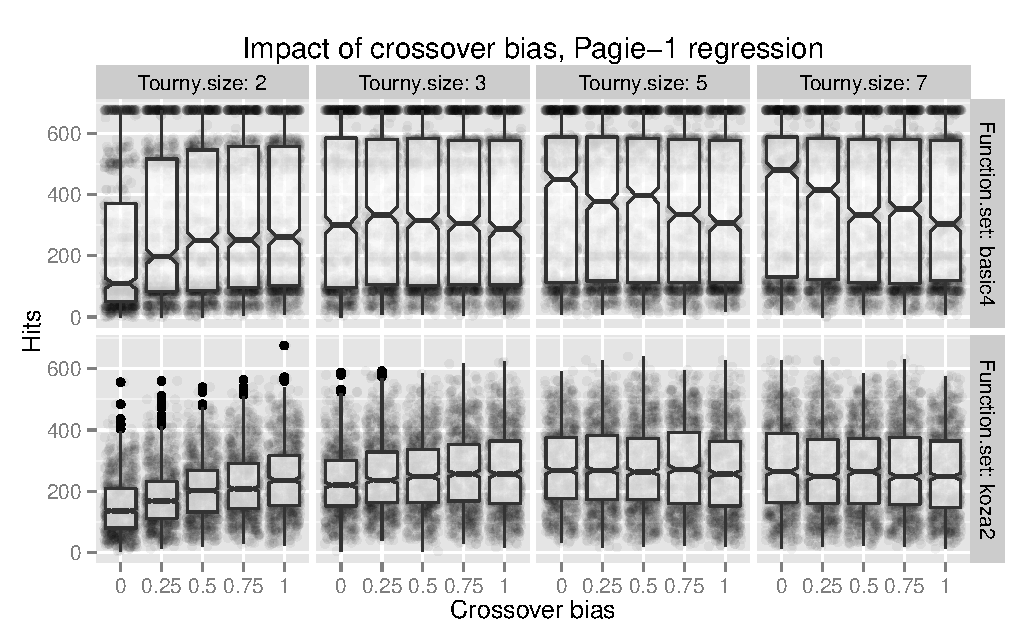
\includegraphics[width=0.45 \textwidth]{Plots/Pagie_1_Hits_vs_Bias_Tournys_FunctionSet.pdf}
\caption{Impact of crossover bias on the number of hits for the Pagie-1 symbolic regression problem, broken out across the four different tournament sizes (2, 3, 5, and 7). The maximum number of possible hits is 676.}
\label{fig:Pagie1Hits_Bias_Tournys_FunctionSet}
\end{figure}

\begin{figure}
\centering
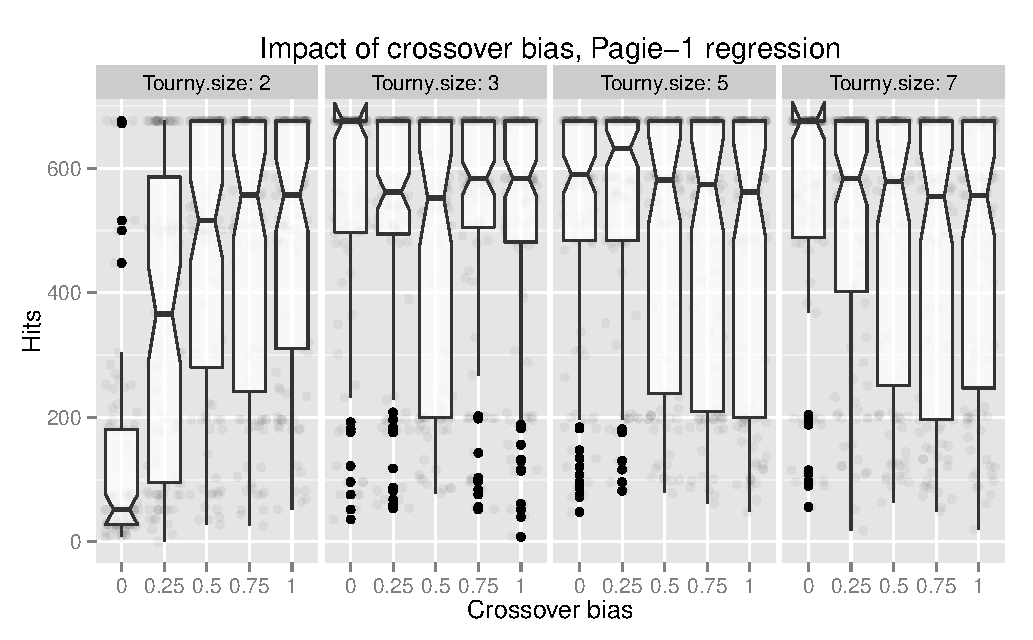
\includegraphics[width=0.45 \textwidth]{Plots/Pagie_1_strong_Hits_vs_Bias_Tournys_FunctionSet.pdf}
\caption{Impact of crossover bias on the number of hits for the Pagie-1 symbolic regression problem, broken out by 
tournament size (2, 3, 5, and 7). These runs use the ``basic4'' function set ($+, -, \times, \div$), no elitism, 
population size 10,240, and Tarpeian bloat control. The maximum number of possible hits is 676.}
\label{fig:Pagie1StrongHits_Bias_Tournys_FunctionSet}
\end{figure}

Focusing on the binary tournament data in Figure~\ref{fig:Pagie1StrongHits_Bias_Tournys_FunctionSet}, the differences between crossover
bias 0.00 (standard subtree crossover) and all the other positive crossover bias values are statistically significant
($p<10^{-12}$), and all of the differences between crossover bias 0.25 and higher biases are significant ($p<0.007$);
however, none of the differences among 0.50, 0.75, and 1.00 are statistically significant. None of the differences for
tournament sizes 3, 5, or 7 are statistically significant, although the difference between crossover biases 0.00 and
1.00 are very close ($p=0.053$) for tournament size 7. This indicates that for binary tournaments, including crossover
bias substantially and significantly improves the hit rate, although all bias rates above 0.25 are very similar. For
tournament size 7, however, it appears that adding crossover bias tends to reduce the hit rate, although in a less
substantial and significant manner.

%> pairwise.wilcox.test(subset(pagie1_strong, Tourny.size==2)$Hits, subset(pagie1_strong, Tourny.size==2)$Bias)
%
%	Pairwise comparisons using Wilcoxon rank sum test 
%
%data:  subset(pagie1_strong, Tourny.size == 2)$Hits and subset(pagie1_strong, Tourny.size == 2)$Bias 
%
%     0       0.25    0.5     0.75   
%0.25 1.7e-13 -       -       -      
%0.5  < 2e-16 0.00639 -       -      
%0.75 < 2e-16 0.00076 1.00000 -      
%1    < 2e-16 0.00037 1.00000 1.00000
%
%P value adjustment method: holm 

Figure~\ref{fig:Pagie1StrongSuccesses} shows the number of successes (runs that exactly solve the problem). Almost none
of these differences are statistically significant, with the major exception being the small number of successes (3)
for binary tournaments without bias, which is significantly different from all the other bias values for binary
tournaments ($p<0.0002$). The one other exception is for tournament size 7, the difference between the number of
successes with crossover biases 0.00 and 1.00 is significant ($p=0.015$).

\begin{figure}
\centering
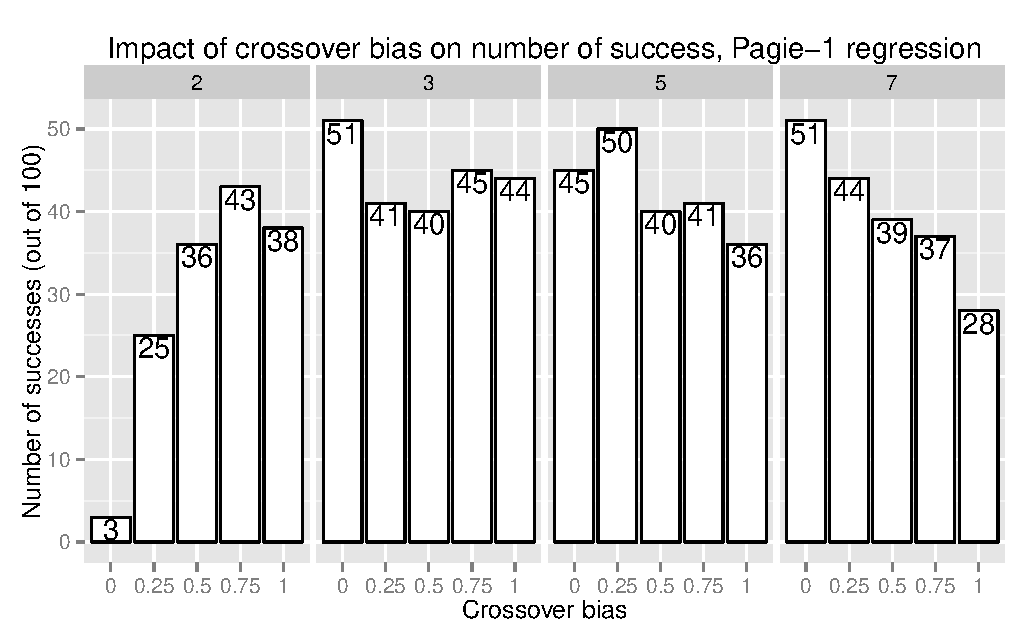
\includegraphics[width=0.45 \textwidth]{Plots/Pagie_1_Strong_Successes_vs_Bias.pdf}
\caption{Impact of crossover bias on the number of successes (runs that exactly solve the problem) for the Pagie-1
symbolic regression problem broken out by tournament size (2, 3, 5, and 7). These runs use the ``basic4'' function set
(just $+, -, \times, \div$), no elitism, population size 10,240, and Tarpeian bloat control.}
\label{fig:Pagie1StrongSuccesses}
\end{figure}

\subsubsection{Sine Problem}

For the sine regression problem, we limited our runs to bias-effective
and non-bias-effective settings as discussed in detail in Section~\ref{sec:Experiments}. 

Figure~\ref{fig:sineBiasResultsStrong} shows the hits results for the sine regression problem using bias-effective settings. All these differences are statistically significant ($p < 10^{-5}$) except for the difference between the bias of 0.75 and 1.00. Figure~\ref{fig:sineBiasFitnessVsGenStrong} also shows the impact of crossover bias over time when using the bias-effective settings; the fitnesses are consistently different throughout the time of the runs, although the differences are shrinking towards the end as many runs find fairly highly fit individuals.

\textbf{Re-do sine figures to use bias-effective and non-bias-effective in titles.}

\begin{figure}
\centering
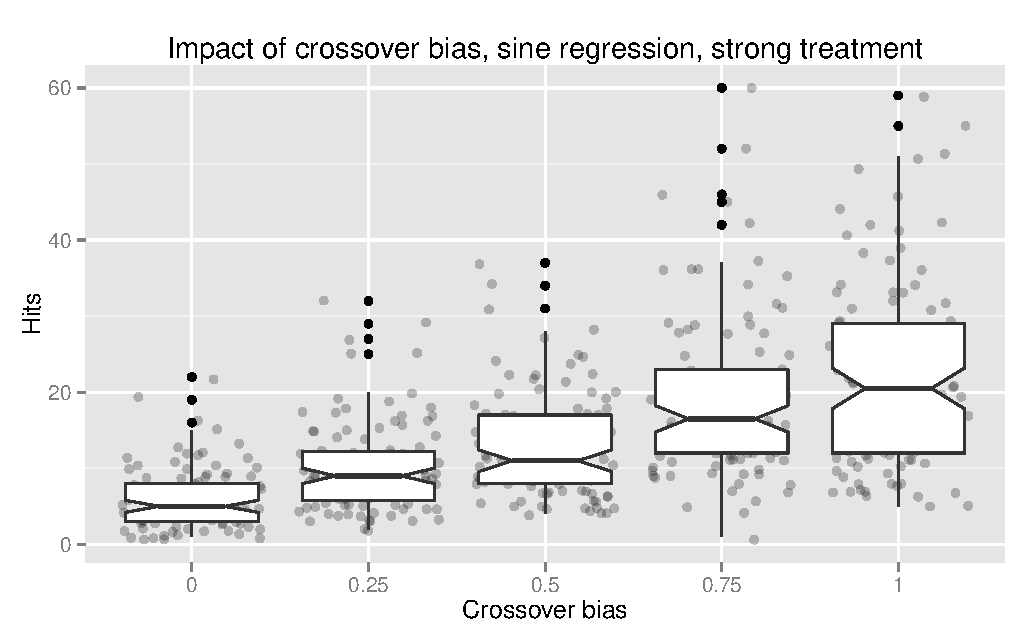
\includegraphics[width=0.45 \textwidth]{Plots/Sine_XO_impact_strong_boxplot.pdf}
\caption{Impact of crossover bias on the sine symbolic regression problem with bias-effective settings.}
\label{fig:sineBiasResultsStrong}
\end{figure}

%> pairwise.wilcox.test(sine_strong_final$Hits, sine_strong_final$Bias)
%
%	Pairwise comparisons using Wilcoxon rank sum test 
%
%data:  sine_strong_final$Hits and sine_strong_final$Bias 
%
%     0       0.25    0.5     0.75  
%0.25 1.9e-07 -       -       -     
%0.5  4.0e-15 0.0017  -       -     
%0.75 < 2e-16 1.2e-12 8.9e-06 -     
%1    < 2e-16 1.3e-13 2.9e-07 0.1938
%
%P value adjustment method: holm 

%> pairwise.wilcox.test(sine_strong_final$Standardized.fitness, sine_strong_final$Bias)
%
%	Pairwise comparisons using Wilcoxon rank sum test 
%
%data:  sine_strong_final$Standardized.fitness and sine_strong_final$Bias 
%
%     0       0.25    0.5     0.75 
%0.25 3.6e-10 -       -       -    
%0.5  < 2e-16 2.7e-05 -       -    
%0.75 < 2e-16 5.0e-14 1.1e-05 -    
%1    < 2e-16 < 2e-16 2.9e-09 0.072
%
%P value adjustment method: holm 

Figure~\ref{fig:sineBiasResultsWeak} shows the results for the sine regression problem using the non-bias-effective 
parameter settings; none of these differences are statistically significant. Figure~\ref{fig:sineBiasFitnessVsGenWeak} also shows the impact of crossover bias over time when using the non-bias-effective settings. \textbf{Say they're all kinda the same.}

\begin{figure}
\centering
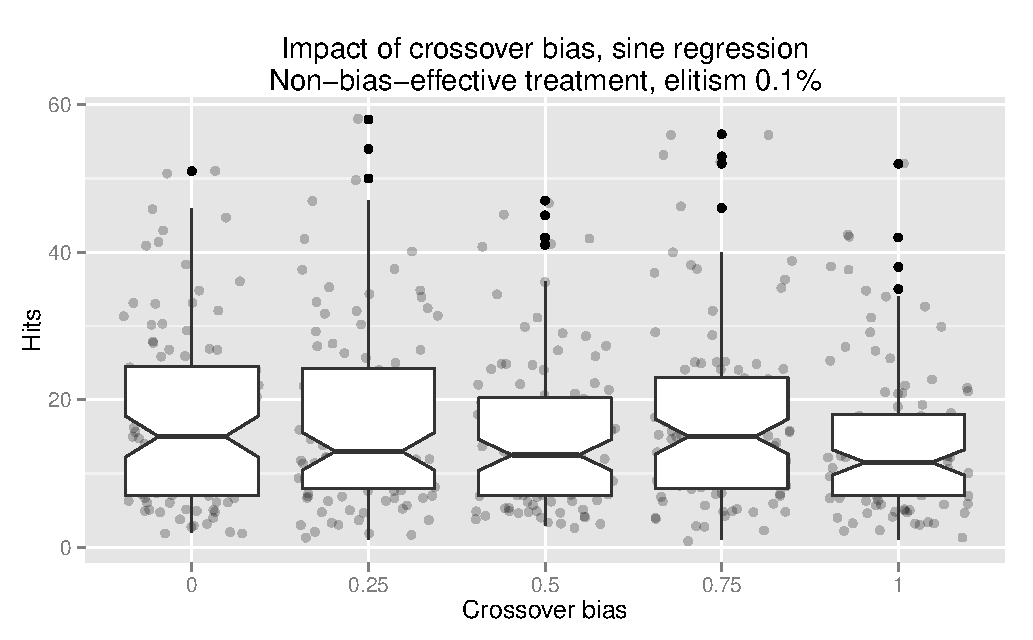
\includegraphics[width=0.45 \textwidth]{Plots/Sine_XO_impact_weak_boxplot.pdf}
\caption{Impact of crossover bias on the sine symbolic regression problem with non-bias-effective settings.}
\label{fig:sineBiasResultsWeak}
\end{figure}

\begin{figure}
\centering
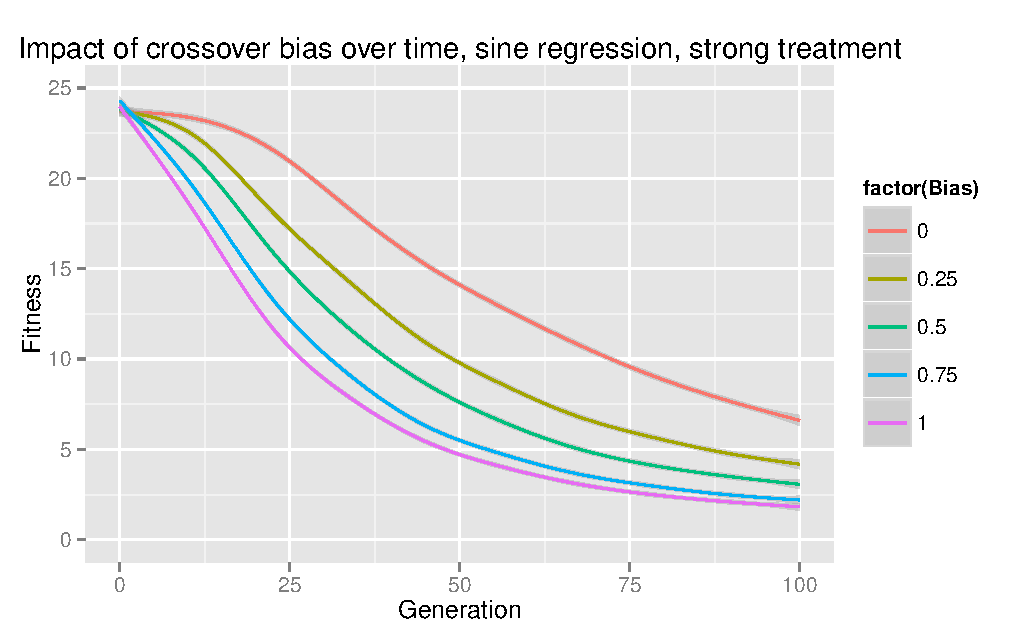
\includegraphics[width=0.45 \textwidth]{Plots/Sine_XO_fitness_vs_gen_strong.pdf}
\caption{Impact of crossover bias on the sine symbolic regression problem with \emph{bias-effective parameter settings}: binary tournaments, no elitism, and 
population size 10,240. \emph{Move this to where we define bias-effective parameters.}}
\label{fig:sineBiasFitnessVsGenStrong}
\end{figure}

\begin{figure}
\centering
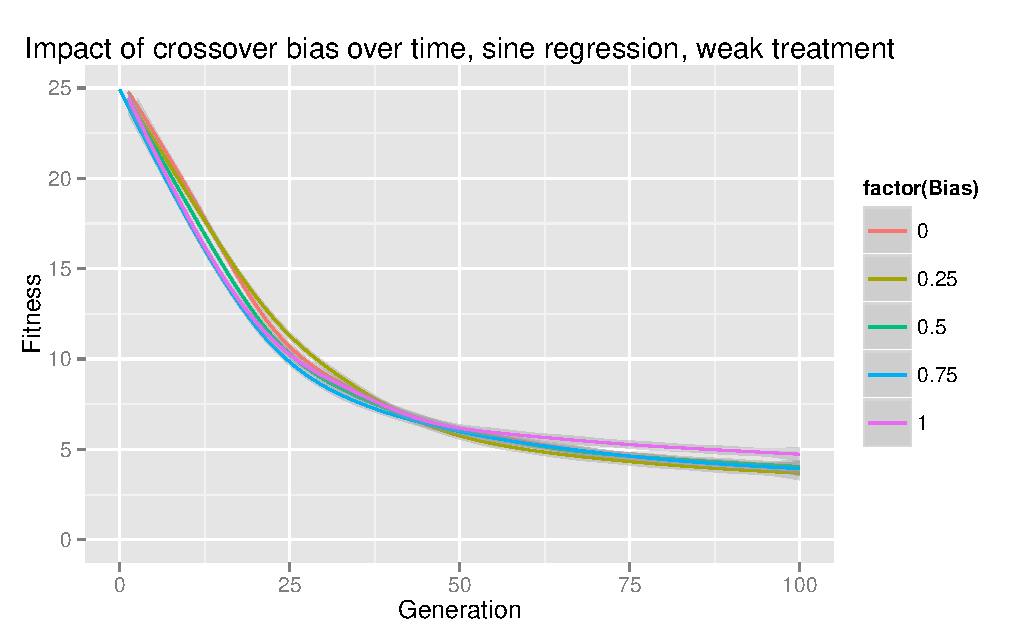
\includegraphics[width=0.45 \textwidth]{Plots/Sine_XO_fitness_vs_gen_weak.pdf}
\caption{Impact of crossover bias on the sine symbolic regression problem with \emph{non-bias-effective parameter settings}: tournament size 7, 0.1\% elitism, and 
population size 1,024.  \emph{Move this to where we define non-bias-effective parameters, combined with the previous figure as a pair of panels.}}
\label{fig:sineBiasFitnessVsGenWeak}
\end{figure}

\section{Discussion} \label{sec:Discussion}

Why does all this happen this way? For example, why does crossover bias have a much stronger effect when using binary
tournaments than when using larger tournament sizes such as 7. One possible explanation is that with large tournaments,
the difference in fitness between the two parents is likely to be closer, because the larger tournaments help ensure
that both parents are from the more highly fit part of the population. Since both of the contributing structures will most likely be from highly fit parents, the resulting offspring will likely obtain similiar fitness as one of these highly fit parent .  To better understand this, Figure~\ref{fig:parentDiffsSine} shows the distribution of relative difference in parent errors in the sine regression 
problem. For each crossover event, the relative difference in parent errors is
\[
	|e_A - e_B] / (e_A + e_B)
\]
where $e_A$ and $e_B$ are the errors of the two chosen parents $A$ and $B$. This has a minimum value of 0 when 
the two errors are the same, and a maximum value approaching 1 for the case where one of the errors is nearly 0. For larger tournament sizes, the difference in fitness drops significantly as the run progresses suggesting that the both of the parents are highly fit. Throughout the run, however, small tournament sizes do not exhibit these changes. (\textbf{not entirely sure what to say here})

\begin{figure}
\centering
\includegraphics[width=0.45 \textwidth]{Plots/Parent_normalized_error_diffs_sine.pdf}
\caption{Plot of the normalized differences in parent errors from some sine runs. \textbf{Explain this}.}
\label{fig:parentDiffsSine}
\end{figure}

We see similar results for the K Landscapes problem, as illustrated in Figure~\ref{fig:parentDiffsKLandscapes}.

\begin{figure}
\centering
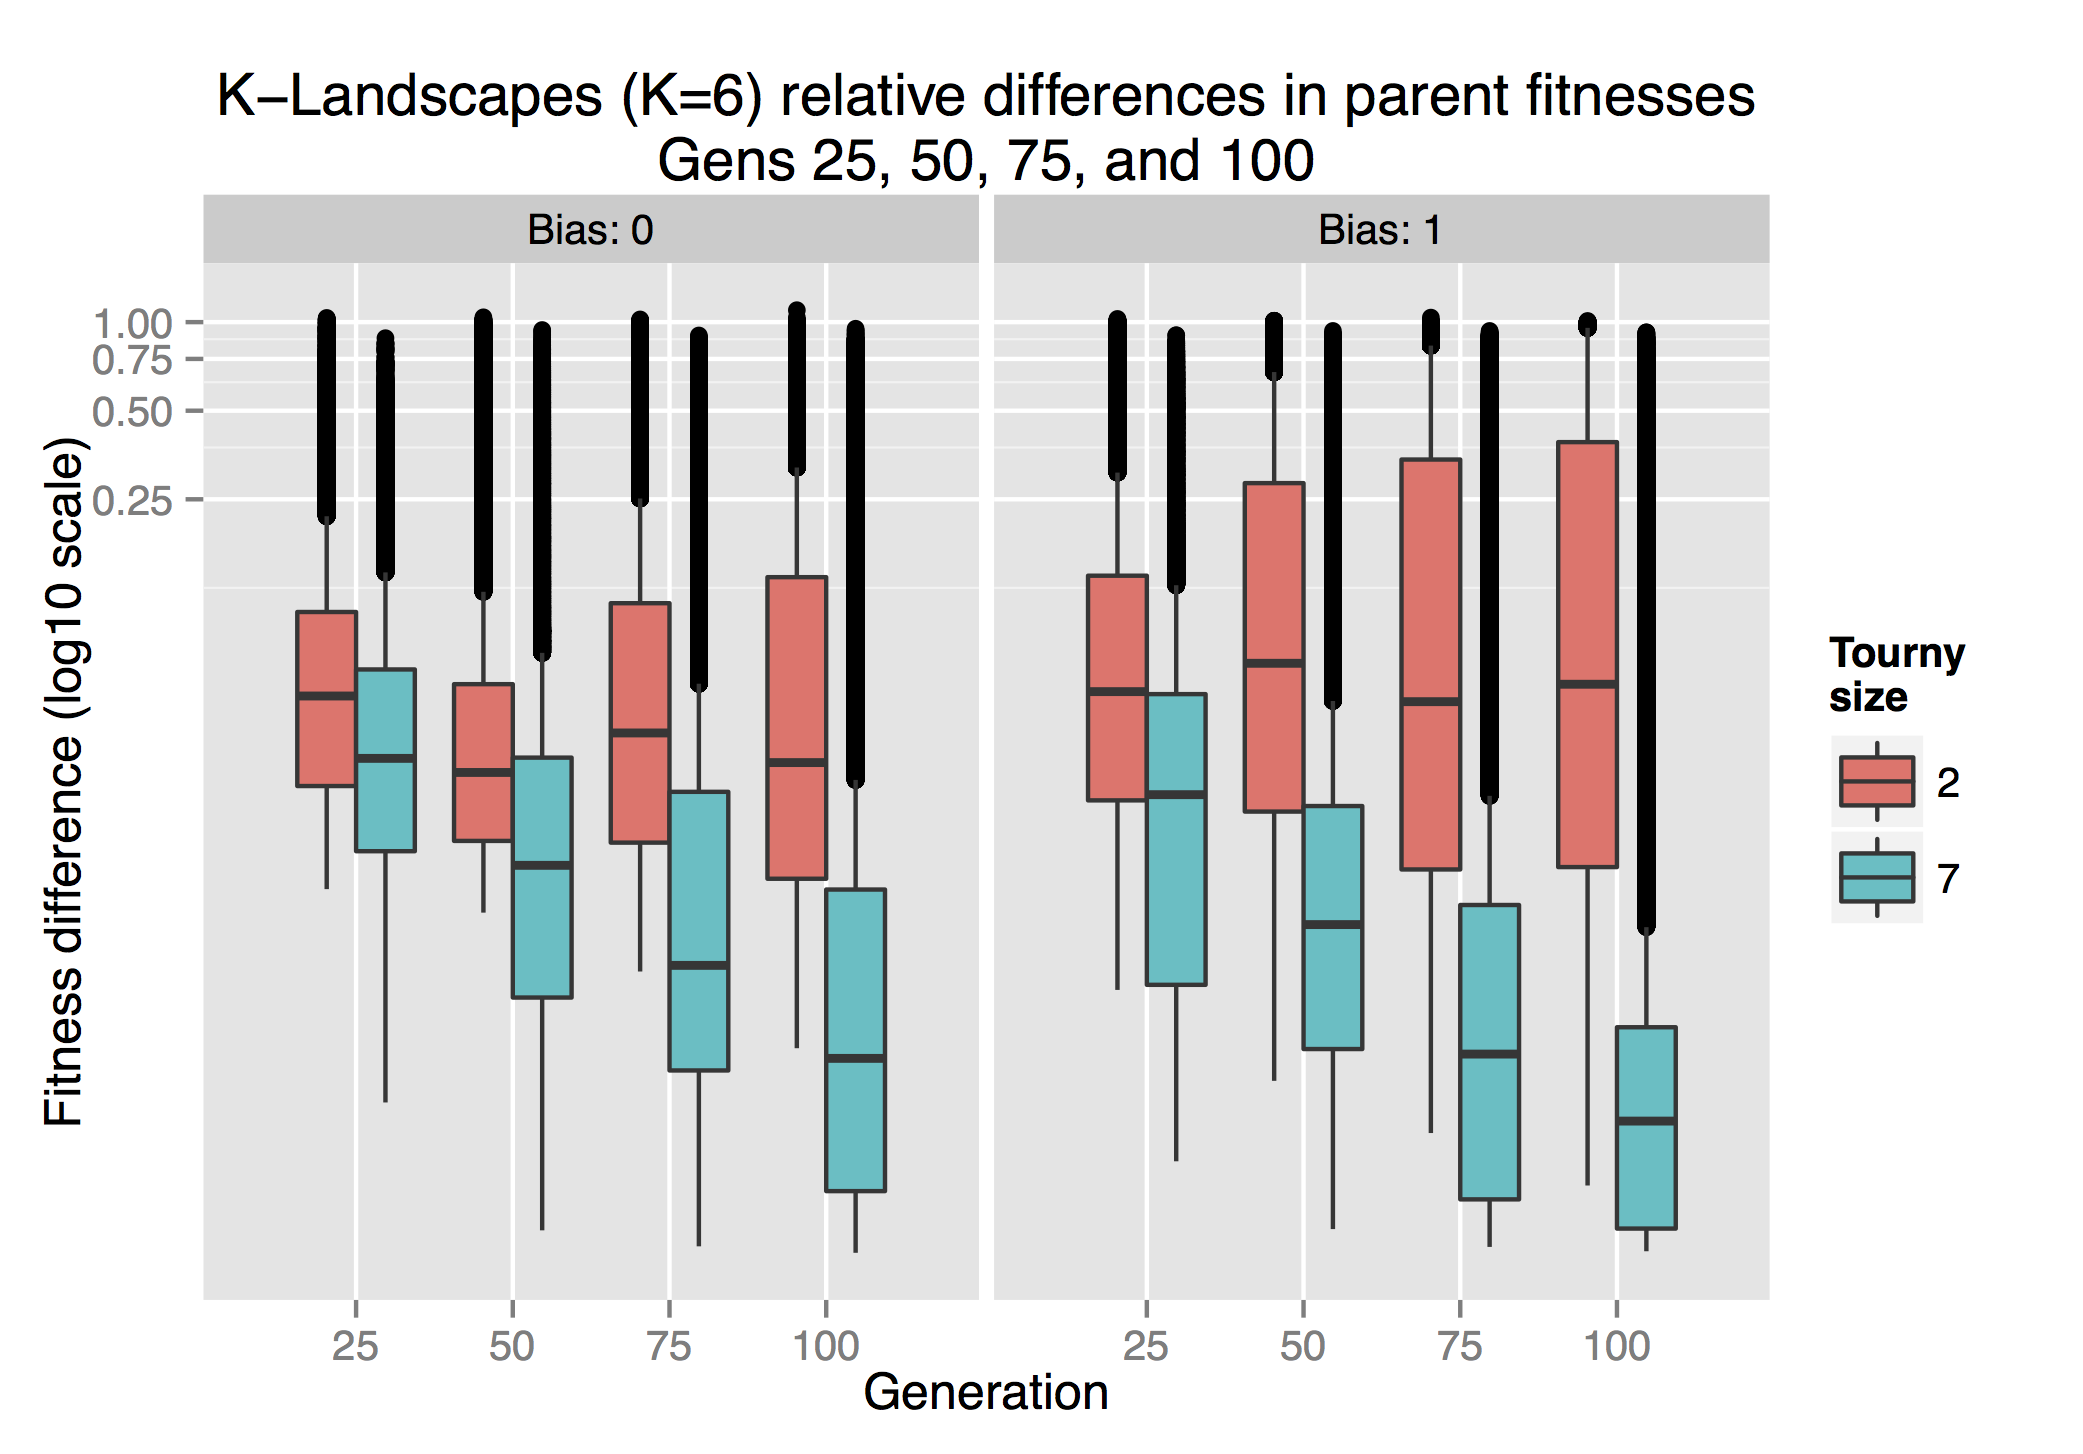
\includegraphics[width=0.45 \textwidth]{Plots/Parent_normalized_fitness_diffs_KLandscapes.pdf}
\caption{Plot of the normalized differences in parent fitnesses from some K Landscape runs. \textbf{Explain this}.}
\label{fig:parentDiffsKLandscapes}
\end{figure}

 Our results also indicate the possibility that crossover bias may increase selection pressure and premature
 convergence (see Figures~\ref{fig:sineBiasFitnessVsGenStrong} and~\ref{fig:sineBiasFitnessVsGenWeak}) \textbf{--
 undesirable behavior, as it encourages a genetic programming run to arrive at a solution too quickly, in the process
 potentially excluding more accurate solutions for a more generalized one}.

\section{Conclusions} \label{sec:Conclusions}

In most of these experiments we found better results with tournament sizes of 7 than with binary tournaments, and in 
general using larger tournaments appears to wash out much of the impact of crossover bias, so there's a fair question 
about whether one should just use larger tournaments and ignore crossover bias. \textbf{How do we respond to this? I 
think the answer is something like ``It doesn't hurt (at least in our experiments), and it sometimes helps, even for 
tournament size 7 and with elitism. For interesting problems, you also don't know in advance what your best parameter 
choices are, so it's at least worth including in your arsenal.''}

One outstanding question is how crossover bias affects generalization. Neither of the published versions 
of the two regression problems specify a validation set, but it's clearly feasible to create validation sets 
for both of those problems and the U.S. Change problem to see what impact, if any, crossover bias has 
on how well evolved solutions generalize to unseen data.

\textbf{Return to the paragraph in the intro about how asymmetries are very common and that these results suggest that we should look at their impact in other EC system.}
In general these 
EC system
asymmetries weren't intentional design goals, but were instead simple artifacts of other system design decisions, and 
the potential impact of these asymmetries has been largely unstudied.

\textbf{I (Nic) suspect that the drop in performance in ORDERTREE is actually quite interesting and might open interesting doors to things like premature
	convergence and need for being able to have a least a little variation in the system for a problem like this. Maybe we
	should talk about that in the "Future work" section?}

% \section*{Acknowledgements}

% Many thanks to the members of the Hampshire College Computational Intelligence Lab for suggestions and feedback as this work developed, with particular thanks to Thomas Helmuth, William LaVaca, and Lee Spector. Thanks also to Thomas Helmuth for introducing us to the U.S. Change problem. Thanks to W. B. Langdon for valuable feedback and numerous suggestions.

\bibliographystyle{acm}
\bibliography{Research_2015}

\end{document}